\documentclass{beamer}

\usepackage{amsmath, amssymb}
\usepackage{tikz-cd}
\usepackage{xcolor}
\usepackage{graphicx}
\usepackage{capt-of}

\title{MAT434: Theory of Mathematical Statistics}
\subtitle{Conditional Distributions \cite{RJA2006}}
\author{\textbf{Miraj Samarakkody}}
\institute{Tougaloo College}
\date{Updated: \today}

\begin{document}

\begin{frame}
    \titlepage
\end{frame}

\begin{frame}
    \frametitle{The Discrete Case}

    If \(X\) and \(Y\) are jointly distributed discrete random variables, the conditional probability that \(X=x_i\) given that \(Y=y_j\) is, if \(p_Y(y_j)>0\), \[
    P(X=x_i|Y=y_j) = \dfrac{P(X=x_i,Y=y_j)}{P(Y=y_j)}= \dfrac{P_{XY}(x_i,y_j)}{p_Y(y_j)}
    \] 
    This probability is defined to be zero if \(p_Y(y_j)=0\).

\end{frame}

\begin{frame}
    \frametitle{Example}

    A fair coin is tossed three times: let \(X\) denote the number of heads on the first toss and \(Y\) the total number of heads. 
    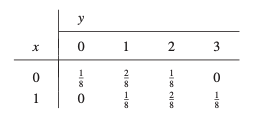
\includegraphics[scale=0.7]{Figures/fig_11.png}\\
    Find the conditional frequency function of \(X\) given \(Y=1\).

\end{frame}

\begin{frame}
    \frametitle{Total Probability}

    The definition of the conditional frequency function can be reexpressed as \[p_{XY}(x,y)=p_{X|Y}(x|y)p_Y(y)\] \pause
    Summing both sides over all values of \(y\), we have an extreamly useful application of the law jof total probability: 
    \[p_X(x)= \sum_Y p_{X|Y}(x|y)p_Y(y)\]
\end{frame}

\begin{frame}
    \frametitle{Example B}

    Suppose that a particle counter is imperfect and independently detects each incoming particle with probability \(p\). If the distribution of the number of incoming particles in a unit time is a Poisson distribution with parameter \(\lambda\), what is the distribution of the number of counted particles? 

\end{frame}

\begin{frame}
    \frametitle{The Continuous Case}

    \begin{block}{Definition}
        
    \end{block}

\end{frame}


\begin{frame}
    \frametitle{References}
    \bibliographystyle{plain} % or another style like unsrt, alpha, etc.
    \bibliography{references}  % omit the .bib extension
\end{frame}



\end{document}